\documentclass[a4paper,12pt, titlepage]{article}
\usepackage{amssymb,amsthm,amsmath} %ams
\usepackage[finnish]{babel} %suomenkielinen tavutus
\usepackage[T1]{fontenc} %skanditavutus
\usepackage[utf8]{inputenc} % skandit utf-8 koodauksella

\usepackage{graphicx} %dokumentti sisältää eps-muotoisia kuvia

\usepackage{changepage}
\usepackage{array}
\usepackage{tabularx}

\usepackage{hyperref}
\hypersetup{
    colorlinks=false,
    pdfborder={0 0 0},
}

\usepackage{float}
\restylefloat{table}


\linespread{1.24} %riviväli 1.5
\sloppy % Vähentää tavutuksen tarvetta, "leventämällä" rivin keskellä olevia välilyöntejä.
\begin{document}

\begin{titlepage}
    \begin{center}
        \vspace*{1cm}
        
        \LARGE
        \textbf{Kakkukaupan verkkokauppa}
        
        \vspace{0.5cm}
        \Large
        Aineopintojen harjoitustyö: Tietokantasovellus
        
        \vspace{1.5cm}
        
        \large
        \textbf{Sami Korhonen} \\
        \text{014021868} \\
        \text{sami.korhonen@helsinki.fi}
        \vfill
        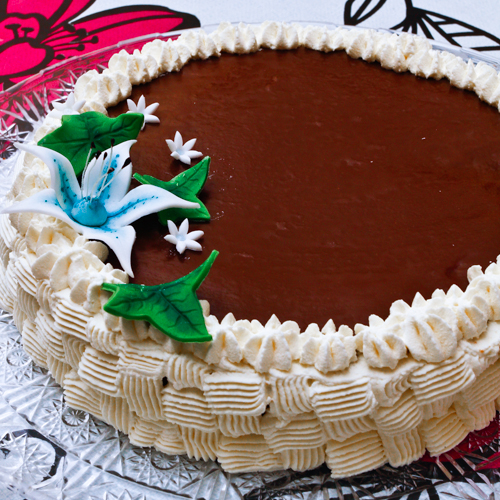
\includegraphics[scale=0.3]{../imgs/kinuskikakku.jpg}\\

		\vfill        
        \normalsize
        Tietojenkäsittelytieteen laitos\\
        Helsingin yliopisto\\
		\large        
        \today
        
    \end{center}
\end{titlepage}

%\maketitle

\tableofcontents
\newpage

\section{Johdanto}
\subsection*{Aihekuvaus}
Kakkukauppa haluaa tehostaa liiketoimintaansa toteuttamalla verkkokaupan, jossa asiakkaat voivat perehtyä tarjontaan ja tehdä tilauksia. Kakkuja on muutamassa eri tuoteryhmässä, kuten hääkakut, synttärikakut ja erikoiskakut. Kakkuja pystyy selaamaan, hakemaan ja lisäämään ostoskoriin. Kakuista saa myös lisätietoja. Palveluun kirjautuneen asiakkaan ostoskori säilyy, vaikka kirjautuisi ulos. Asiakas pystyy myös muuttamaan omia tietojaan ja poistamaan käyttäjätunnuksensa. 

Yhdessä tilauksessa voi olla useampia erilaisia kakkuja, mutta toimituspäivä on kaikille tilauksen tuotteille sama. Tilaukset voi maksaa laskulla tai tilisiirrolla. Tilatut tuotteet voidaan joko noutaa Kakkukaupasta tai toimittaa asiakkaan osoitteeseen. 

Sovelluksessa on työntekijälle tehtyjä ominaisuuksia. Työntekijä pystyy lisäämään, muuttamaan ja poistamaan tuotteita. Lisäksi admin-käyttäjä pystyy muokkaamaan muiden tilien käyttäjätyyppejä ja poistamaan näitä. Työntekijöille olisi myös mahdollista laajentaa toimintoja tilausten muokkaamista varten. 

\subsection*{Sovelluksen tarkoitus}
Sovelluksen tarkoitus on toimia apuvälineenä Kakkukaupan ja asiakkaan välisessä kaupankäynnissä. Sen ei ole tarkoitus ylläpitää tuotteiden saldoja, eikä varsinaisesti arkistoida menneitä tilauksia. Nämä ominaisuudet olisi laajennettavissa, mutta näitä varten olis järkevämpi toteuttaa erilliset järjestelmät. Esimerkiksi maksutapahtumat tapahtuvat laskulla tai tilisiirrolla, eikä sovellukseen ole luotu esimerkiksi verkkopankkimaksamista tietoturvasyistä johtuen. Sovelluksen on tarkoitus lähettää tehdystä tilauksesta sähköposti asiakkaalle ja työntekijälle, jotta tilauksen käsitely voi edetä. Sähköpostin lähettämistä ei kuitenkaan ole tässä harjoitustyössä toteutettu ilkivallan välttämiseksi.

\subsection*{Sovelluksen toteutus}
Tietokantasovellus on toteutettu PHP-kielellä, sen tietokantana toimii MySQL ja se on pystytetty tietojenkäsittelytieteen laitoksen users-palvelimelle. Lähtökohtaisesti sovellus on suunniteltu toimivaksi MySQL tietokannalla, eikä muiden tietokantojen tukea ole juurikaan ajateltu. Tietokantasovellus ei vaadi selaimen tukea ohjelmointikielille, joten sen tulisi pyöriä vähäisemmälläkin selainvarustelulla täysin normaalisti.

\section{Järjestelmän yleiskuva}
\subsection{Käyttötapauskaavio}
\hfill

\noindent
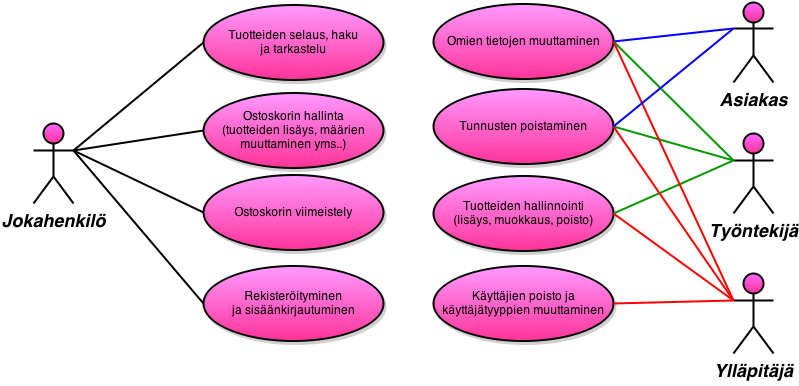
\includegraphics[keepaspectratio, width=\textwidth]{kaaviot/kayttotapauskaavio.png}
\subsection{Käyttäjäryhmät}
\subsubsection*{Jokahenkilö}
Jokahenkilö on kuka tahansa Kakkukaupan verkkokaupan tunnistamaton vierailija tai kirjautunut käyttäjä. Kaikilla käyttäjäryhmillä on myös jokahenkilön oikeudet.
\subsubsection*{Asiakas}
Asiakas on Kakkukaupan verkkokauppaan kirjautunut henkilö. Asiakkaalla on tunnus 	(sähköpostiosoite) ja salasana kirjautumista varten. Asiakkaalla on myös muita tarpeellisia tietoja, kuten osoite ja puhelinnumero. Asiakkaan ostoskori säilyy, vaikka verkkokaupasta kirjautuisi ulos välillä. Lisäksi käyttäjän tiedot täyttyvät kassasivulle automaattisesti tilausta tehdessä.
\subsubsection*{Työntekijä}
Työntekijä on Kakkukaupan työntekijä. Työntekijällä on vastaavat ominaisuudet kuin asiakkaallakin, mutta hänellä pystyy hallinnoimaan lisäksi tuotteita.
\subsubsection*{Ylläpitäjä}
Ylläpitäjä, eli admin, on käyttäjä, jolla on työntekijän oikeuksien lisäksi esimerkiksi mahdollisuus muuttaa käyttäjätyyppejä ja poistaa käyttäjiä.

\subsection{Käyttötapauskuvaukset}
\subsubsection*{Jokahenkilön käyttötapaukset}

Tuotteiden selaus
\begin{adjustwidth}{2.5em}{0pt}
Kuka tahansa voi selata ja hakea tuotteita sekä tarkastella tuotteiden tarkempia tietoja. Tuotteita voi selata kategorioiden mukaan, tai hakea hakusanoilla. Jokaisesta tuotteesta voi myös nähdä erillisen tuotesivun, jossa selitetään tuotteesta yksityiskohtaisemmin.
\end{adjustwidth}
\hfill

\noindent
Tuotteen lisääminen ostoskoriin
\begin{adjustwidth}{2.5em}{0pt}
Kuka tahansa voi lisätä ostoskoriinsa tuotteita haluamansa määrän mukaan.
\end{adjustwidth}
\hfill

\noindent
Tuotteen poistaminen ostoskorista
\begin{adjustwidth}{2.5em}{0pt}
Kuka tahansa voi poistaa omasta ostoskoristaan tuotteen, tai tyhjentää koko ostoskorin.
\end{adjustwidth}
\hfill

\noindent
Ostoskorin määrien muuttaminen
\begin{adjustwidth}{2.5em}{0pt}
Kuka tahansa voi muokata ostoskorissaan olevien tuotteiden määriä.
\end{adjustwidth}
\hfill

\noindent
Rekisteröityminen
\begin{adjustwidth}{2.5em}{0pt}
Kuka tahansa pystyy rekisteröitymään Kakkukaupan asiakkaaksi, mutta samalla sähköpostiosoitteella ei voi olla kahta käyttäjätunnusta samanaikaisesti.
\end{adjustwidth}
\hfill

\noindent
Sisäänkirjautuminen
\begin{adjustwidth}{2.5em}{0pt}
Kuka tahansa pystyy kirjautumaan sisään, mikäli käyttäjältä löytyy käyttäjätunnus ja salasana.
\end{adjustwidth}
\hfill

\noindent
Tilauksen viimeistely
\begin{adjustwidth}{2.5em}{0pt}
Kuka tahansa pystyy viimeistelemään ostoskorin ja tekemään tilauksen, mikäli ostoskorin ja tilauksen tiedot ovat kunnossa.
\end{adjustwidth}

\subsubsection*{Asiakkaan käyttötapaukset}
Omien tietojen muutttaminen
\begin{adjustwidth}{2.5em}{0pt}
Sisäänkirjautunut henkilö pystyy muokkaamaan omia tietojaan, kuten salasanansa, osoitteensa, sähköpostinsa tai puhelinnumeronsa. 
\end{adjustwidth}
\hfill

\noindent
Käyttäjätunnuksen poistaminen
\begin{adjustwidth}{2.5em}{0pt}
Sisäänkirjautunut henkilö pystyy poistamaan oman käyttäjätunnuksensa.
\end{adjustwidth}
\hfill

\noindent
Asiakkaalla on näiden lisäksi myös kaikki jokahenkilön käyttötapaukset.

\subsubsection*{Työntekijän käyttötapaukset}
Tuotteen lisääminen
\begin{adjustwidth}{2.5em}{0pt}
Työntekijä pystyy lisäämään verkkokauppaan uusia tuotteita.
\end{adjustwidth}
\hfill

\noindent
Tuotteen muokkaaminen
\begin{adjustwidth}{2.5em}{0pt}
Työntekijä pystyy muokkaamaan verkkokaupassa olevia tuotteita.
\end{adjustwidth}
\hfill

\noindent
Tuotteen poistaminen
\begin{adjustwidth}{2.5em}{0pt}
Työntekijä pystyy poistamaan verkkokaupassa olevia tuotteita.
\end{adjustwidth}
\hfill

\noindent
Työntekijällä on näiden lisäksi myös kaikki asiakkaan käyttötapaukset.


\subsubsection*{Ylläpitäjän käyttötapaukset}
Käyttäjätyyppien muuttaminen
\begin{adjustwidth}{2.5em}{0pt}
Ylläpitäjä (admin) pystyy muuttamaan käyttäjien käyttäjätyyppejä.
\end{adjustwidth}
\hfill

\noindent
Käyttäjien poistaminen
\begin{adjustwidth}{2.5em}{0pt}
Ylläpitäjä (admin) pystyy poistamaan käyttäjiä.
\end{adjustwidth}
\hfill

\noindent
Ylläpitäjällä on näiden lisäksi myös työntekijän käyttötapaukset.

\section{Järjestelmän tietosisältö}
\subsection{Käsitekaavio}
\hfill

\begin{center}
\noindent
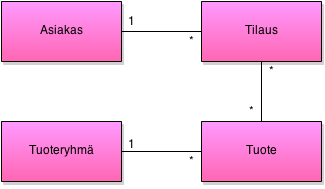
\includegraphics[keepaspectratio, scale=0.8]{kaaviot/kasitekaavio.png}
\end{center}
\subsection{Tietokohteet}
\subsubsection*{Tietokohde: Tuote}
\begin{table}[H]
\begin{tabularx}{\textwidth}{|p{2.5cm}|p{3.5cm}|X|}
\hline
\bf{Attribuutti} & \textbf{Arvojoukko}	& \textbf{Kuvailu}  \\ \hline
Nimi           & Merkkijono, max. 80 merkkiä   & Tuotteen nimi            \\ \hline
Hinta		   & Desimaaliluku                 & Tuotteen hinta euroina   \\ \hline
Kuvaus         & Merkkijono, max. 3000 merkkiä & Tuotteen tarkempi kuvaus \\ \hline
Kuva           & Merkkijono, max. 20 merkkiä   & Tuotteen kuvatiedoston nimi \\ \hline
\end{tabularx}
\end{table}

\subsubsection*{Tietokohde: Tuoteryhma}
\begin{table}[H]
\begin{tabularx}{\textwidth}{|p{2.5cm}|p{3.5cm}|X|}
\hline
\bf{Attribuutti} & \textbf{Arvojoukko}	& \textbf{Kuvailu}  \\ \hline
Nimi		& Merkkijono, max. 50 merkkiä   & Tuoteryhmän nimi, esimerkiksi: ”Hääkakut” \\ \hline
\end{tabularx}
\end{table}

\subsubsection*{Tietokohde: Tilaus}
\begin{table}[H]
\begin{tabularx}{\textwidth}{|p{2.5cm}|p{3.5cm}|X|}
\hline
\bf{Attribuutti} & \textbf{Arvojoukko}	& \textbf{Kuvailu}  \\ \hline
Tilausvaihe   & Merkkijono, max. 50 merkkiä  & Tilausvaihe, esim. ”Avoin”, ”Odottaa maksua” tai ”Toimitettu” \\ \hline
Tilauspäivä   & Päivämäärä                   & Päivämäärä, jolloin tilaus on tehty                           \\ \hline
Toimituspäivä & Päivämäärä                   & Päivämäärä, jolloin tilaus on määrä toimittaa asiakkaalle     \\ \hline
Toimitustapa  & Merkkijono, max. 20 merkkiä  & Toimitustapa, esim. ”Nouto” tai ”Toimitus”                    \\ \hline
Maksutapa     & Merkkijono, max. 20 merkkiä  & Maksutapa, esim. ”Lasku tai ”Tilisiirto”                      \\ \hline
\end{tabularx}
\end{table}

\subsubsection*{Tietokohde: Kayttaja}
\begin{table}[H]
\begin{tabularx}{\textwidth}{|p{2.5cm}|p{3.5cm}|X|}
\hline
\bf{Attribuutti} & \textbf{Arvojoukko}	& \textbf{Kuvailu}  \\ \hline
Etunimi              & Merkkijono, max. 80 merkkiä  & Kayttajan etunimi                                   \\ \hline
Sukunimi             & Merkkijono, max. 80 merkkiä  & Kayttajan sukunimi                                  \\ \hline
Sahkoposti           & Merkkijono, max. 80 merkkiä  & Kayttajan sähköpostiosoite                          \\ \hline
Puhelin              & Merkkijono, max. 15 merkkiä  & Kayttajan puhelinnumero                             \\ \hline
Osoite               & Merkkijono, max. 80 merkkiä  & Kayttajan katuosoite, esim. ”Tietokantakuja 13”     \\ \hline
Postinumero          & Merkkijono, max. 5 merkkiä   & Postinumero, sisältää vain numeroita, esim. ”00100” \\ \hline
Paikkakunta          & Merkkijono, max. 30 merkkiä  & Postitoimipaikka, esim. ”Helsinki”                  \\ \hline
Salasana             & Merkkijono, max. 128 merkkiä & Kayttajan salasana (kryptattuna 128 merkkiä)        \\ \hline
\end{tabularx}
\end{table}

\newpage
\section{Relaatiotietokantakaavio}
\hfill

\noindent
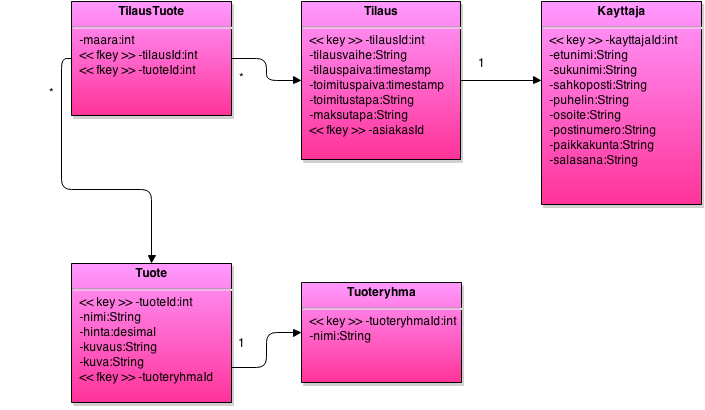
\includegraphics[keepaspectratio, width=\textwidth]{kaaviot/relaatiotietokantakaavio.png}

\section{Järjestelmän yleisrakenne}
Tämä tietokantasovellus on tehty noudattaen MVC-mallia. Kontrollerit sijaitsevat juurihakemistossa, näkymät hakemistossa \verb|views| ja hakemistosta \verb|models| löytyy mallit. Hakemistosta \verb|libs| löytyy yleishyödyllisiä tiedostoja (\verb|common.php| ja \verb|tietokanta.php|). MySQL-serveriin liittyvät tiedostot ovat \verb|sql|-hakemistossa, jotta tietokannan alasajo ja pystyttäminen olisi helppoa. Kansiosta \verb|imgs| löytyy sivuilla käytettävät kuvat. Malliluokat sisältäviä tiedostoja lukuunottamatta kaikki tiedostot on kirjoitettu pienellä alkukirjaimella. Kontrollerit on jätetty juurihakemistoon, jotta verkkokaupan asiakkaat voivat kopioida osoiteriviltä mahdollisimman nättejä osotteita esimerkiksi halutessaan näyttää tuotetta ystävälleen.

Hakemistosta löytyy myös muutamia ylimääräisiä tiedostoja, joita ei hyödynnetä tässä tietokantasovelluksessa. Nämä liittyvät kurssin muihin tehtäviin ja ne on sijoitettu hakemistoon \verb|others|. Näitä tiedostoja ovat esimerkiksi \verb|html-demo| -hakemiston sisältö ja \verb|listatesti.php|.

\section{Käyttöliittymä ja järjestelmän komponentit}
\hfill

\noindent
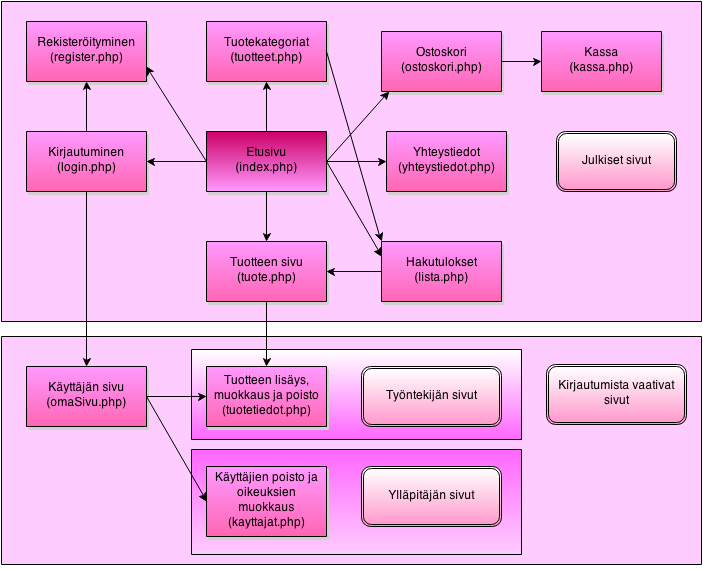
\includegraphics[keepaspectratio, width=\textwidth]{kaaviot/kayttoliittymayhteydet.png}
\hfill

\noindent
Käytännössä sivustolla on käytössä navigaatiopalkki, josta pääsee tuotteen tietoja lukuunottamatta kaikialle, mihin kaavion mukaan pääsee etusivulta. Kirjautumista ei juurikaan vaadita, mutta esimerkiksi navigaatiopalkin näkymä riippuu hieman siitä, onko käyttäjä kirjautunut sisään vai ei. Ostoskorin ja kassan käyttö on myös hieman erilaista kirjautuneelle käyttäjälle.

\section{Asennustiedot}
MySQL-tietokannan ja PHP-tuen asentamisen jälkeen sovelluksen voi ottaa käyttöön uudella palvelimella kohtuullisen yksinkertaisesti. Sovelluksen tiedostot tulee siirtää tai kopioida hakemistoon, johon pääsee internetin kautta. Tällä hetkellä tiedostot ovat users-palvelimen htdocs-kansiossa. Kansiorakenne ja tiedostot tulee säilyttää ennallaan toiminnan varmistamiseksi. Kun tiedostot on siirretty uuteen sijaintiin tulee tiedostoon libs/tietokanta.php asettaa uuden tietokannan osoite ja tunnukset. Tämänhetkisessä tiedostossa on esimerkki, jota vastaavalla tavalla saa tietokannan asetettua uuteen palvelimeen. Lopuksi tietokannassa tulee suorittaa sql-hakemistosta löytyvät \verb|create-tables.sql| ja \verb|add-test-data.sql| -tiedostot juuri tässä järjestyksestä. Tämän jälkeen sovelluksen tulisi olla käytettävissä.

\section{Käynnistys- / käyttöohje}
Verkkokaupan käyttäminen on hyvin intuitiivista. Verkkokaupan etusivu löytyy osoitteesta: \\
\url{http://samkorho.users.cs.helsinki.fi/kakkukauppa} \\
\hfill

\noindent
Monet ominaisuudet ovat käytössä kirjautumatta sisään, mutta sisään voi kirjautua esimerkiksi seuraavilla tunnuksilla: 

\begin{table}[H]
\begin{tabularx}{\textwidth}{|X|X|X|}
\hline
\bf{Käyttäjätunnus} & \textbf{Salasana}	& \textbf{Käyttäjätyyppi}  \\ \hline
admin@kakku.fi   & admin & admin \\ \hline
jobbari@kakku.fi   & jobbari & tyontekija \\ \hline
asiakas@kakku.fi   & asiakas & asiakas \\ \hline

\end{tabularx}
\end{table}

\noindent
Näillä tunnuksilla pääsee kirjautumaan sisään osoitteessa: \\
\url{http://samkorho.users.cs.helsinki.fi/kakkukauppa/login.php}

\section{Testaus, tunnetut bugit ja puutteet ja jatkokehitysideat}
Sovelluksen testaaminen on tapahtunut manuaalisesti, joskaan suurempia hankaluuksia ei ole ollutkaan. PHP:n tuoreimpia virheitä seuraamalla on pystynyt ratkaisemaan ongelmien lähteet kohtalaisen kätevästi. Pääasiallisesti sivuja on katseltu Chromium- ja Chrome-selaimilla.

Tällä hetkellä ei ole tiedossa varsinaisia bugeja, joskin verkkosivun ulkoasu saattaa vaihdeilla selaimen ja resoluution mukaan. Esimerkiksi matkapuhelinten selaimet saattavat kadottaa värit ja rikkoa koko rakenteen. Kaikki toteutetut ominaisuudet ovat toimineet ainakin jossain vaiheessa, mutta automaattisten testien puuttuessa on mahdollista, että jokin ominaisuus on hajonnut ja jäänyt huomaamatta.

Puutteeita verkkokaupassa voisivat olla aikaisempien tilausten seuraaminen ja arkistointi, sekä yhteydenoton puute. Sovelluksen olisi käyttöön otettaessa tarkoitus lähettää sähköpostia asiakkaalle ja työntekijälle tehdystä tilauksesta, mutta tämän on päätetty jättää toteuttamatta mahdollisen ilkivallan välttämiseksi. Tietoturvan osalta saattaisi olla muutenkin paranneltavaa, mikäli sovellus haluttaisiin ottaa käyttöön esimerkiksi verkkopankkimaksamista silmällä pitäen. Lisäksi olisi kätevämpää, jos admin-käyttäjä pystyisi hakemaan muita käyttäjiä muokatakseen näiden käyttäjätyyppeja, mutta ajanpuutteen vuoksi tästä on luovuttu.

Ohjelmaa on kehitetty pitäen mielessä mahdollisia jatkokehitysideoita. Näitä ovat esimerkiksi erilaisten tuotevariaatioiden (esim. koko, väri tai maku) toteuttaminen, tilaushistorian ylläpito, tuotteiden varastotilanteen selvittäminen ja muutamat laajennukset työntekijäpalveluihin ja tuotetietoihin. 

\section{Omat kokemukset}
Palvelinpuolen tietokantaohjelmointia olen hieman tehnyt aiemmin Java:lla, jonka vuoksi halusin valita PHP:n oppiakseni uutta. Projektin tekeminen on ollut sekä mielekästä ja hermoja raastavaa. Toisinaan PHP:n ja HTML:n käyttö tuntuu hyvin luontevalta, joskin välillä on hankaluuksia muistaa syntaksia ja sovelluksen rakennetta. Minusta on ollut hyvin mielenkiintoista päästä tekemään itse valitsemaani aihetta, jonka tekemisestä on mahdollisesti hyötyä jatkossa. Tietokannan käyttö on täyttänyt tällä kurssilla hyvin sen aukon käytännön osaamisesta, minkä Tietokantojen perusteet jättävät.

\section{Liitteet}
Create table, drop table ja lausekkeet testidatan luomiseen sisältävät SQL-tiedostot löytyvät repositoriosta hakemistosta sql:
\begin{verbatim}
create-tables.sql
drop-tables.sql
add-test-data.sql
\end{verbatim}

\end{document}